\chapter{Introducción a la teoría de grafos}

Se dice que la Teoría de Grafos tiene su origen en 1736, cuando Euler dio una 
solución al problema (hasta entonces no resuelto) de los siete puentes de 
Königsberg: ¿existe un camino que atraviese cada uno de los puentes exactamente 
una vez?  

\begin{figure}[h]
\captionsetup{font=scriptsize}
\caption{Dibujo de los 7 puentes de Königsberg}
\centering
\includegraphics[scale=.6]{images}
\end{figure}

Para probar que no era posible, Euler sustituyó cada región por un nodo y cada 
puente por una arista, creando el primer grafo que fuera modelo de un problema
matemático. 

\begin{center}
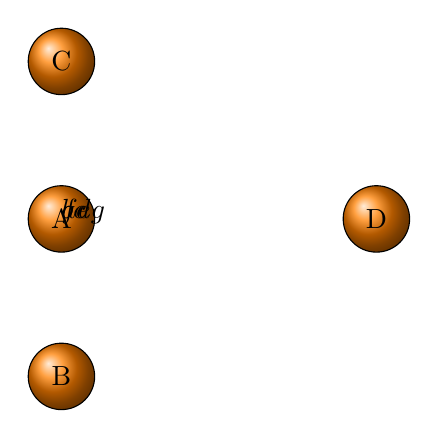
\begin{tikzpicture}
     \GraphInit[vstyle=Shade]
     \begin{scope}
     \tikzstyle{every node} = [draw,
                               shape          = circle,
                               ball color     = orange,
                               text           = black,
                               minimum size   = 24 pt]
     \node (A) at (0, 0){A};
     \node (B) at (0,-2){B};
     \node (C) at (0, 2){C};
     \node (D) at (4, 0){D};
     \end{scope}
     \begin{scope}
     \tikzset{EdgeStyle/.append style = {bend left}}
     \Edge[label=$b$](A)(B)
     \Edge[label=$c$](A)(C)
     \end{scope}
     \begin{scope}
     \tikzset{EdgeStyle/.append style = {bend right}}
     \Edge[label=$a$](A)(B)
     \Edge[label=$d$](A)(C)
     \end{scope}
     \Edge[label=$f$](B)(D)
     \Edge[label=$e$](A)(D)
     \Edge[label=$g$](C)(D)
  \end{tikzpicture}
\end{center}

Desde entonces, se ha ido desarrollando esta metodología hasta 
convertise en los últimos años en una herramienta importante en áreas del 
conocimiento muy variadas como, por ejemplo: la Investigación Operativa, la 
Computación, la Ingeniería Eléctrica, la Geografía y la Química. Es por ello que, 
además, se ha erigido como una nueva disciplina matemática, que generalmente 
asociada a las ramas de Topología y Álgebra.

La utilidad de los grafos se basa en su gran poder de abstracción y una
representación muy clara de cualquier relación, lo que facilita enormemente 
tanto la fase de modelado como la de resolución de cualquier problema. Gracias a
la Teoría de Grafos se han desarrollado una gran variedad de algoritmos y métodos
de decisión que podemos implementar a través de lenguajes funcionales y permiten 
automatizar la resolución de muchos problemas, a menudo  tediosos de resolver a mano.

\comentario{Pendiente de ampliar la introducción conforme se vaya escribiendo
los módulos.}

\minitoc

\section{Definición de grafo}

En primer lugar, vamos a introducir terminología básica en el desarrollo de la Teoría de 
Grafos.

\begin{definicion}
  Un \textbf{grafo} $G$ es un par $(V,A)$, donde $V$ es el conjunto de los
  vértices (o nodos) y $A$ el de las aristas. Un \textbf{grafo dirigido} es un
  grafo en el que las aristas están orientadas.
  
  En muchas aplicaciones de los grafos las aristas llevan asociada información adicional.
  En ese caso hablaremos de \textbf{grafos etiquetados}. Si esa información es numérica,
  diremos que es el valor de la etiqueta es el peso de la arista y diremos que $G$ es un
  \textbf{grafo ponderado}.
\end{definicion}

\begin{definicion}
  Una \textbf{arista} de un grafo $G=(V,A)$, es un par de elementos
  de $V$. En el caso de los grafos dirigidos, denotaremos a las aristas por 
  \textbf{arcos} y el par será ordenado. Es decir, para dos vértices $v,v'$ de un grafo
  dirigido, $(v,v')$ y $(v',v)$ no son la misma arista, mientras que en un grafo 
  dirigido sí lo serían.

  Una \textbf{arista de un grafo etiquetado}, $G=(V,A)$, es una tupla de la forma
  $(v,v',e)$ donde $v,v' \in V$ y $e$ es la información que contiene la arista.
  Si el grafo es no dirigido, las aristas  $(v,v',e)$ y  $(v',v,e)$ son iguales y si
  el grafo es dirigido son distintas. 
\end{definicion}

% Idea: v es adyacente a v' si desde v' podemos llegar de un salto a v.

\begin{definicion}
  Dado un grafo $G=(V,A)$, diremos que un vértice $v \in V$ es \textbf{adyacente}
  a $v' \in V$ si $(v',v) \in A$. 

  En el caso de los grafos etiquetados, diremos que un vértice $v \in V$ es 
  adyacente a $v' \in V$ si existe alguna etiqueta $e$ tal que $(v',v,e) \in A$.
\end{definicion}

\begin{definicion}
  Si en un grafo dirigido se permiten aristas repetidas, lo llamaremos 
  \textbf{multigrafo}. Si no se permiten, lo llamaremos \textbf{grafo regular}.
\end{definicion}

\begin{nota}
  Denotaremos por $|V|$ al número de vértices y por $|A|$ al número de aristas
  del grafo $(V,A)$.
\end{nota}

\begin{ejemplo}

  Sea $G = (V,A)$ un grafo no dirigido con $V = \{a,b,c,d\}$ y
  $A = \{\allowbreak(a,b), \allowbreak (a,c), \allowbreak (b,d), \allowbreak (d,d)\}$.
  En este grafo, los vértices $a,d$ son adyacentes a $b$.

  \begin{center},
  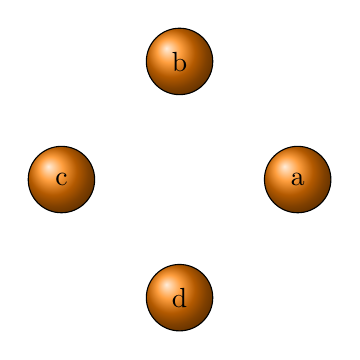
\begin{tikzpicture}
  \SetVertexNoLabel
  \tikzstyle{every node} = [draw, 
                            shape = circle,
                            ball color=orange,
                            minimum size = 24pt]
  \GraphInit [vstyle = Shade]
  \node (a) at (0:1.5){a};
  \node (b) at (90:1.5){b};
  \node (c) at (180:1.5){c};
  \node (d) at (270:1.5){d};
  \Edge (a)(b)
  \Edge (a)(c)
  \Edge (b)(d)
  \Edge (d)(d);
  \end{tikzpicture}
  \end{center}

  Sea $G = (V,A)$ un grafo dirigido con $V = \{a,b,c,d\}$ y
  $A = \{\allowbreak(a,b),\allowbreak (a,c),\allowbreak (b,d),\allowbreak
  (d,d)\}$.  En este grafo, solo el vértice $d$ es adyacente a $b$.

  \begin{center}
  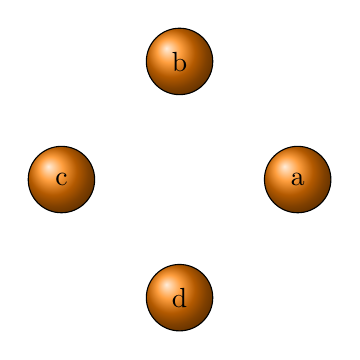
\begin{tikzpicture}
  \SetVertexNoLabel
  \tikzset{EdgeStyle/.style = {{->},
                               thick,%
                               double           = orange,
                               double distance  = 1pt}} 
  \begin{scope}
  \tikzstyle{every node} = [draw, 
                            shape = circle,
                            ball color=orange,
                            minimum size = 24pt]
  \node (a) at (0:1.5){a};
  \node (b) at (90:1.5){b};
  \node (c) at (180:1.5){c};
  \node (d) at (270:1.5){d};
  \Edge (a)(b)
  \Edge (a)(c)
  \Edge (b)(d)
  \end{scope}
  \Loop[dist=1cm,dir=SO,label=$ $,labelstyle=above](d) 
  \end{tikzpicture}
  \end{center}

  Sea $G = (V,A)$ un grafo dirigido ponderado con $V = \{a,b,c,d\}$ y
  $A = \{\allowbreak (a,b,2), \allowbreak (a,c,4),\allowbreak
  (b,d,2),\allowbreak (d,d,3)\}$.  En este grafo, los vértices $a,d \in V$ son
  adyacentes a $b$.
  \begin{center}
  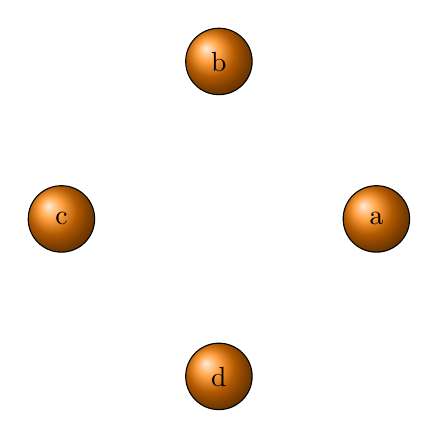
\begin{tikzpicture}
  \SetVertexNoLabel
  \tikzset{EdgeStyle/.style = {{->},thick,double = orange,double distance = 1pt}}
  \begin{scope}

  \tikzstyle{every node} = [draw, 
                            shape = circle,
                            ball color=orange,
                            minimum size = 24pt]
  \node (a) at (  0:2){a};
  \node (b) at ( 90:2){b};
  \node (c) at (180:2){c};
  \node (d) at (270:2){d};
  \end{scope}
  \tikzstyle{every node} = [pos=0.25]
  \Edge [label={4}](a)(c)
  \Edge [label={2}](b)(d)
  \tikzstyle{every node} = [fill=white,pos=0.5,text = black]
  \Edge [label={2}](a)(b)
  \Loop[dist=1.5cm,dir=SO,label=3](d) 
  \end{tikzpicture}
  \end{center}
\end{ejemplo}

\begin{definicion} 
  Si en un grafo dirigido se permiten aristas que vayan de un vértice en sí mismo, 
  entonces el grafo se dice \textbf{pseudografo}. Si las aristas de un grafo no son dirigidas
  pero sí se pueden repetir aristas (y lazos), lo llamaremos \textbf{multigrafo}.
\end{definicion}

\section{El TAD de los grafos}

\label{sec:TAD_grafos}

En esta sección, nos planteamos la tarea de implementar las
definiciones presentadas anteriormente en un lenguaje funcional. En nuestro
caso, el lenguaje que utilizaremos será Haskell. Definiremos el Tipo Abstracto
de Dato (TAD) de los grafos y daremos algunos ejemplos de posibles
representaciones de grafos con las que podremos trabajar.

La primera definición de grafo que vamos a implementar es para grafos finitos no
dirigidos y no ponderados. Si consideramos un grafo finito cualquiera 
$G = (V,A)$, podemos ordenar el conjunto de los vértices y representarlo como 
$V = \{v_1, \dots, v_n\}$ con $n = |V|$.

En primer lugar, necesitaremos crear un tipo \texttt{(Grafo)} cuya definición sea compatible
con la entidad matemática que representa y que nos permita definir las operaciones que 
necesitamos para trabajar con los grafos. Estas operaciones son:

\begin{code}
creaGrafo   :: (Vertice,Vertice) -> [(Vertice,Vertice)] -> Grafo
adyacentes  :: Grafo -> Vertice -> [Vertice]
nodos       :: Grafo -> [Vertice]
aristas     :: Grafo -> [(Vertice,Vertice)]
aristaEn    :: Grafo -> (Vertice,Vertice) -> Bool
\end{code}
donde:

\begin{itemize}
\item \texttt{(creaGrafo cs as)} es un grafo tal que sus vértices vendrán dados
              por el par de cotas \texttt{cs} y las aristas por la lista \texttt{as}.
\item \texttt{(nodos g)} es la lista de todos los nodos del grafo \texttt{g}.
\item \texttt{(aristas g)} es la lista de las aristas del grafo \texttt{g}.
\item \texttt{(adyacentes g v)} es la lista de los vértices adyacentes al nodo
             \texttt{v} en el grafo \texttt{g}.
\item \texttt{(aristaEn g a)} se verifica si \texttt{a} es una arista del grafo
             \texttt{g}.
\end{itemize}

\begin{nota}
  Las funciones que aparecen en la especificación del TAD no dependen 
  de la representación que elijamos.
\end{nota}

\begin{ejemplo}

Veamos un ejemplo de creación de grafo y su representación gráfica

\begin{code}
creaGrafo (1,5) [(1,2),(1,3),(1,5),(2,4),
                 (2,5),(3,4),(3,5),(4,5)]
\end{code}

\begin{center}
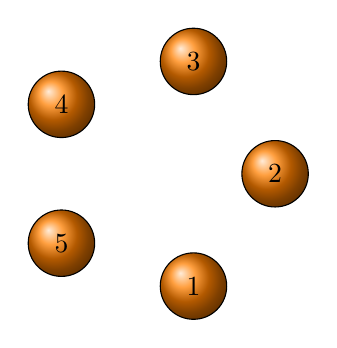
\begin{tikzpicture}
   \tikzstyle{every node} = [draw, shape =circle,ball color=orange,minimum size = 24pt]
   \GraphInit[vstyle=Shade]
   \node (v0) at (4*72:1.5) {1};
   \node (v1) at (   0:1.5) {2};
   \node (v2) at (  72:1.5) {3};
   \node (v3) at (2*72:1.5) {4};
   \node (v4) at (3*72:1.5) {5};
   \Edge(v0)(v1)
   \Edge(v0)(v2)
   \Edge(v0)(v4)
   \Edge(v1)(v3)
   \Edge(v1)(v4)
   \Edge(v2)(v3)
   \Edge(v2)(v4)
   \Edge(v3)(v4);
\end{tikzpicture}
\end{center}
\end{ejemplo}

A lo largo del trabajo, utilizaremos tres representaciones de grafos: grafos
como vectores de adyacencia, grafos como matrices de adyacencia y grafos como
listas de aristas.

Las tres representaciones tienen tanto ventajas como inconvenientes. En general,
las representaciones como vectores de adyacencia y como matrices de adyacencia
son más eficientes, sin embargo, la representación como lista de aristas es más
dinámica y permite trabajar más fácilmente con algoritmos que impliquen un 
cambio en el grafo. 

Informalmente, cuando un grafo tiene un gran número de aristas, diremos que
el grafo es \textbf{denso} y cuando tiene pocas, diremos que es 
\textbf{disperso}. En algunos libros, esta idea se formaliza, diciendo que 
un grafo $G=(V,A)$ es disperso cuando $|A|<|V|·log(|V|)$ y denso en caso 
contrario. Normalmente, la representación como matriz es mejor para grafos
densos y la representación como vector mejor para grafos dispersos.

\subsection{Grafos como vectores de adyacencia}

\entrada{GrafoConVectorDeAdyacencia}

\subsection{Grafos como matrices de adyacencia}

\entrada{GrafoConMatrizDeAdyacencia}

\subsection{Grafos como listas de aristas}

\entrada{GrafoConListaDeAristas}

\section{Generadores de grafos}

Hemos necesitado crear dos generadores de grafos, uno para las representaciones
como vectores de adyacencia y como matrices de adyacencia y otro para la 
representación como listas de aristas.

\subsection{Generador de grafos como vectores y matrices de adyacencia}

\entrada{GeneradorGrafosArray}

\subsection{Generador de grafos como listas de aristas}

\entrada{GeneradorGrafosListas}

\section{Ejemplos de grafos}

\entrada{EjemplosGrafosLista}

\section{Definiciones y propiedades}

\entrada{DefinicionesYPropiedadesLista}

\section{Ejemplo de módulo Haskell}
\entrada{ITG}

%%% Local Variables:
%%% mode: latex
%%% TeX-master: "MD_en_Haskell"
%%% End:
